\section{Cloud Computing}

Im folgenden Unterkapitel werden die Grundlagen und eine Definition des Cloud Computing erarbeitet. Hierbei werden die Grundlegenden Konzepte, Bereitstellungsmodelle und Abstraktionsebenen des Cloud Computing erläutert.

\subsection{Was ist Cloud Computing}

Das \ac{NIST}, auf dessen Definition sich in der Literatur häufig bezogen wird \cite[Vgl.][S. 4f]{Reinheimer2018} hat Cloud Computing wie folgt definiert: Cloud Computing ist ein Modell der Zurverfügungstellung von Computing Ressourcen (z.B. Netzwerke, Server, Speicher, Anwendungen und Services). Diese werden über das Netzwerk zu Verfügung gestellt um mit geringem Managementaufwand schnell freigegeben und bereitgestellt werden können \cite[Vgl.][S. 2]{Mell2011}\cite[Vgl.][S. 5]{Reinheimer2018}.

\begin{figure}{H}
    \centering
    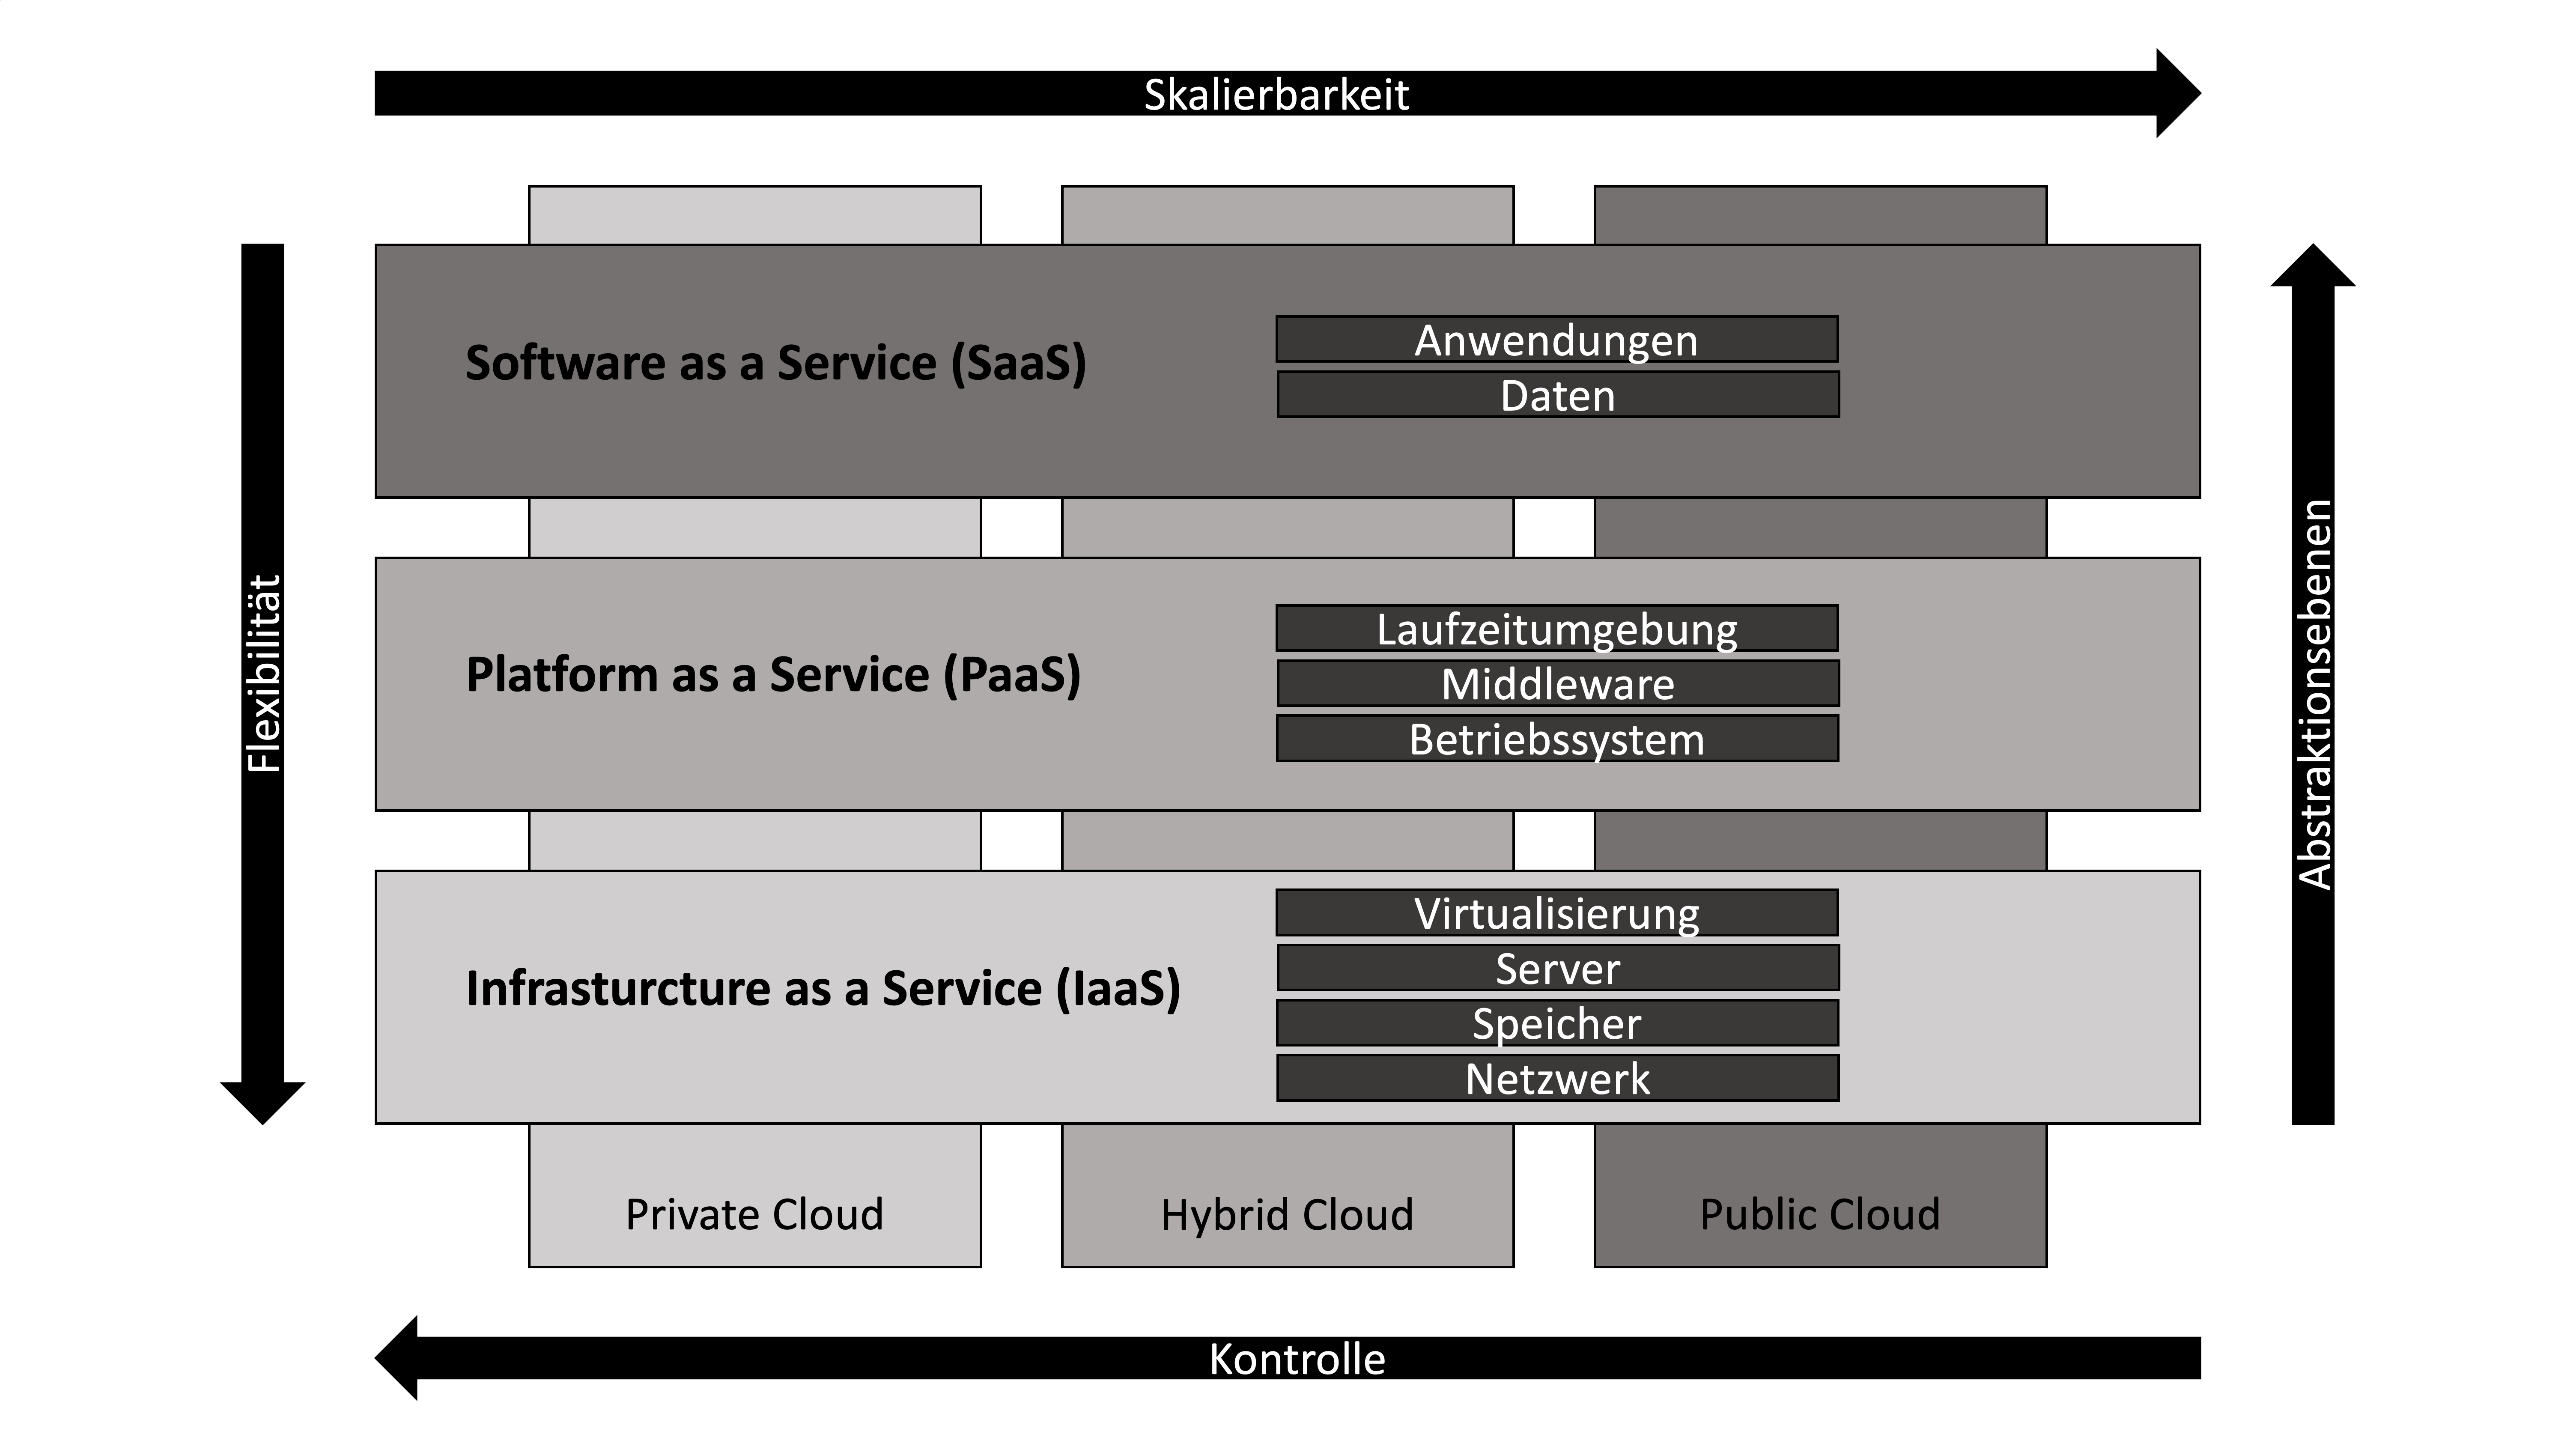
\includegraphics[height=0.4\textwidth]{xaas.png}
    \caption{Eine Übersicht der Cloud Service Modelle \cite[Eigene Darstellung nach][S. 33]{Maenhaut2016}\cite[Ergänzt durch][]{Toroman2018}}
    \label{fig:XaaS}
\end{figure}

Nach Hentschel und Leyh (2018), Zhao (2014), Maenhaut (2016) und Surianarayanan (2019) kann man Cloud Services grundsätzlich in drei Abstraktionsebenen einteilen. Diese sind \textbf{\ac{SaaS}}, \textbf{\ac{PaaS}} und \textbf{\ac{IaaS}}, welche auch zu \ac{XaaS} zusammengefasst werden \cite[Vgl.][S. 9]{Reinheimer2018}\cite[Vgl.][S. 143f]{Zhao2014}\cite[Vgl.][S. 32ff]{Maenhaut2016} und \cite[Vgl.][S. 226ff]{Surianarayanan2019}.

Die in Abbildung \ref{fig:XaaS} dargestellte unterste der drei genannten Abstraktionsschichten ist \ac{IaaS}, welche die Basisinfrastruktur, wie zum Beispiel Netzwerk, Server oder Speicher, bereitstellt.

Diese Infrastruktur kann sowohl physisch als auch virtuell zur Verfügung gestellt werden \cite[Vgl.][S. 9f]{Reinheimer2018}. Die darüberliegend dargestellte Schicht ist \ac{PaaS}, welche zu der Infrastrukturebene zusätzlich noch eine Basis zur Anwendungsentwicklung bietet, indem zum Beispiel bereits ein Betriebssystem und Middleware und eine Laufzeitumgebung bereitgestellt werden \cite[Vgl.][S. 10]{Reinheimer2018}. Die oberste Abstraktionsebene ist \ac{SaaS}, welche standardisierte Anwendungen zur Verfügung stellt und somit ohne Verwaltung der zugrundeliegenden Ressourcen genutzt werden kann. Die Bereitstellung der Anwendung wird vom Provider übernommen.
\cite[Vgl.][S. 11]{Reinheimer2018}.

Generell wird die Cloud darüber hinaus in drei Organisationsdimensionen eingeteilt \cite[Vgl. auch im Folgenden][S. 7ff]{Reinheimer2018}:
\begin{itemize}
\item \textbf{Private Cloud:} Die Private Cloud bietet die exklusive Nutzung durch eine Organisation. Die IT-Infrastruktur einer Private Cloud kann entweder im Unternehmenseigenen Rechenzentrum untergebracht oder auch von Dienstleistern bereitgestellt werden.
\item \textbf{Public Cloud:} In der Public Cloud ist die Infrastruktur für mehr Anwender zugänglich und muss geteilt werden. Dafür muss als Anwender oft auch nur für die tatsächlich genutzte Leistung gezahlt werden. Da die Infrastruktur jedoch gleichzeitig von vielen genutzt wird, ist zum Beispiel der Betrieb von sicherheitskritischen Anwendungen schwierig.
\item \textbf{Hybrid Cloud:} Die Hybrid Cloud bildet eine kombinierte Anwendung aus der Public Cloud und der Private Cloud. Diese bietet dem Anwender die Möglichkeit gewisse Anwendungen in die Public Cloud auszulagern, ohne die Vorteile der Private Cloud für sicherheitsrelevante Anwendungen aufgeben zu müssen. Als weiterer möglicher Aspekt kann bei einem Hybrid Cloud Modell die Rechenleistung der Private Cloud bei Spitzenlast durch die Public Cloud für nicht sicherheitskritische Anwendungen erweitert werden. 
\end{itemize}

\pagebreak

\subsection{Entwicklung des Cloud Computing}

Die Entwicklung des Cloud Computing und dessen Vorgängerkonzepte is bis in die 90er Jahre zurückzuführen. Ein von Hentschel und Leyh (2018) hervorgehobener Vorgänger ist das sogenannte Grid Computing. Damit war bereits eine dezentrale Ressourcenkontrolle mir standardisierten Protokollen und Schnittstellen realisiert. Das Cloud Computing bietet vergleichbare Eigenschaften, jedoch rückt der Fokus hier auf wirtschaftliche Kriterien und die Zentralisierung von Ressourcen zum Beispiel in Rechenzentren \cite[Vgl.][S. 5f]{Reinheimer2018}.

Salesforce war eines der ersten Unternehmen, welches 1999 Anwendungen über eine Webseite bereitgestellt hat, gefolgt von \ac{AWS} in 2002, welche Speicher und Rechenleistung als Services bereitstellten \cite[Vgl.][S. 17f]{Srivastava2018}.

\begin{figure}[H]
    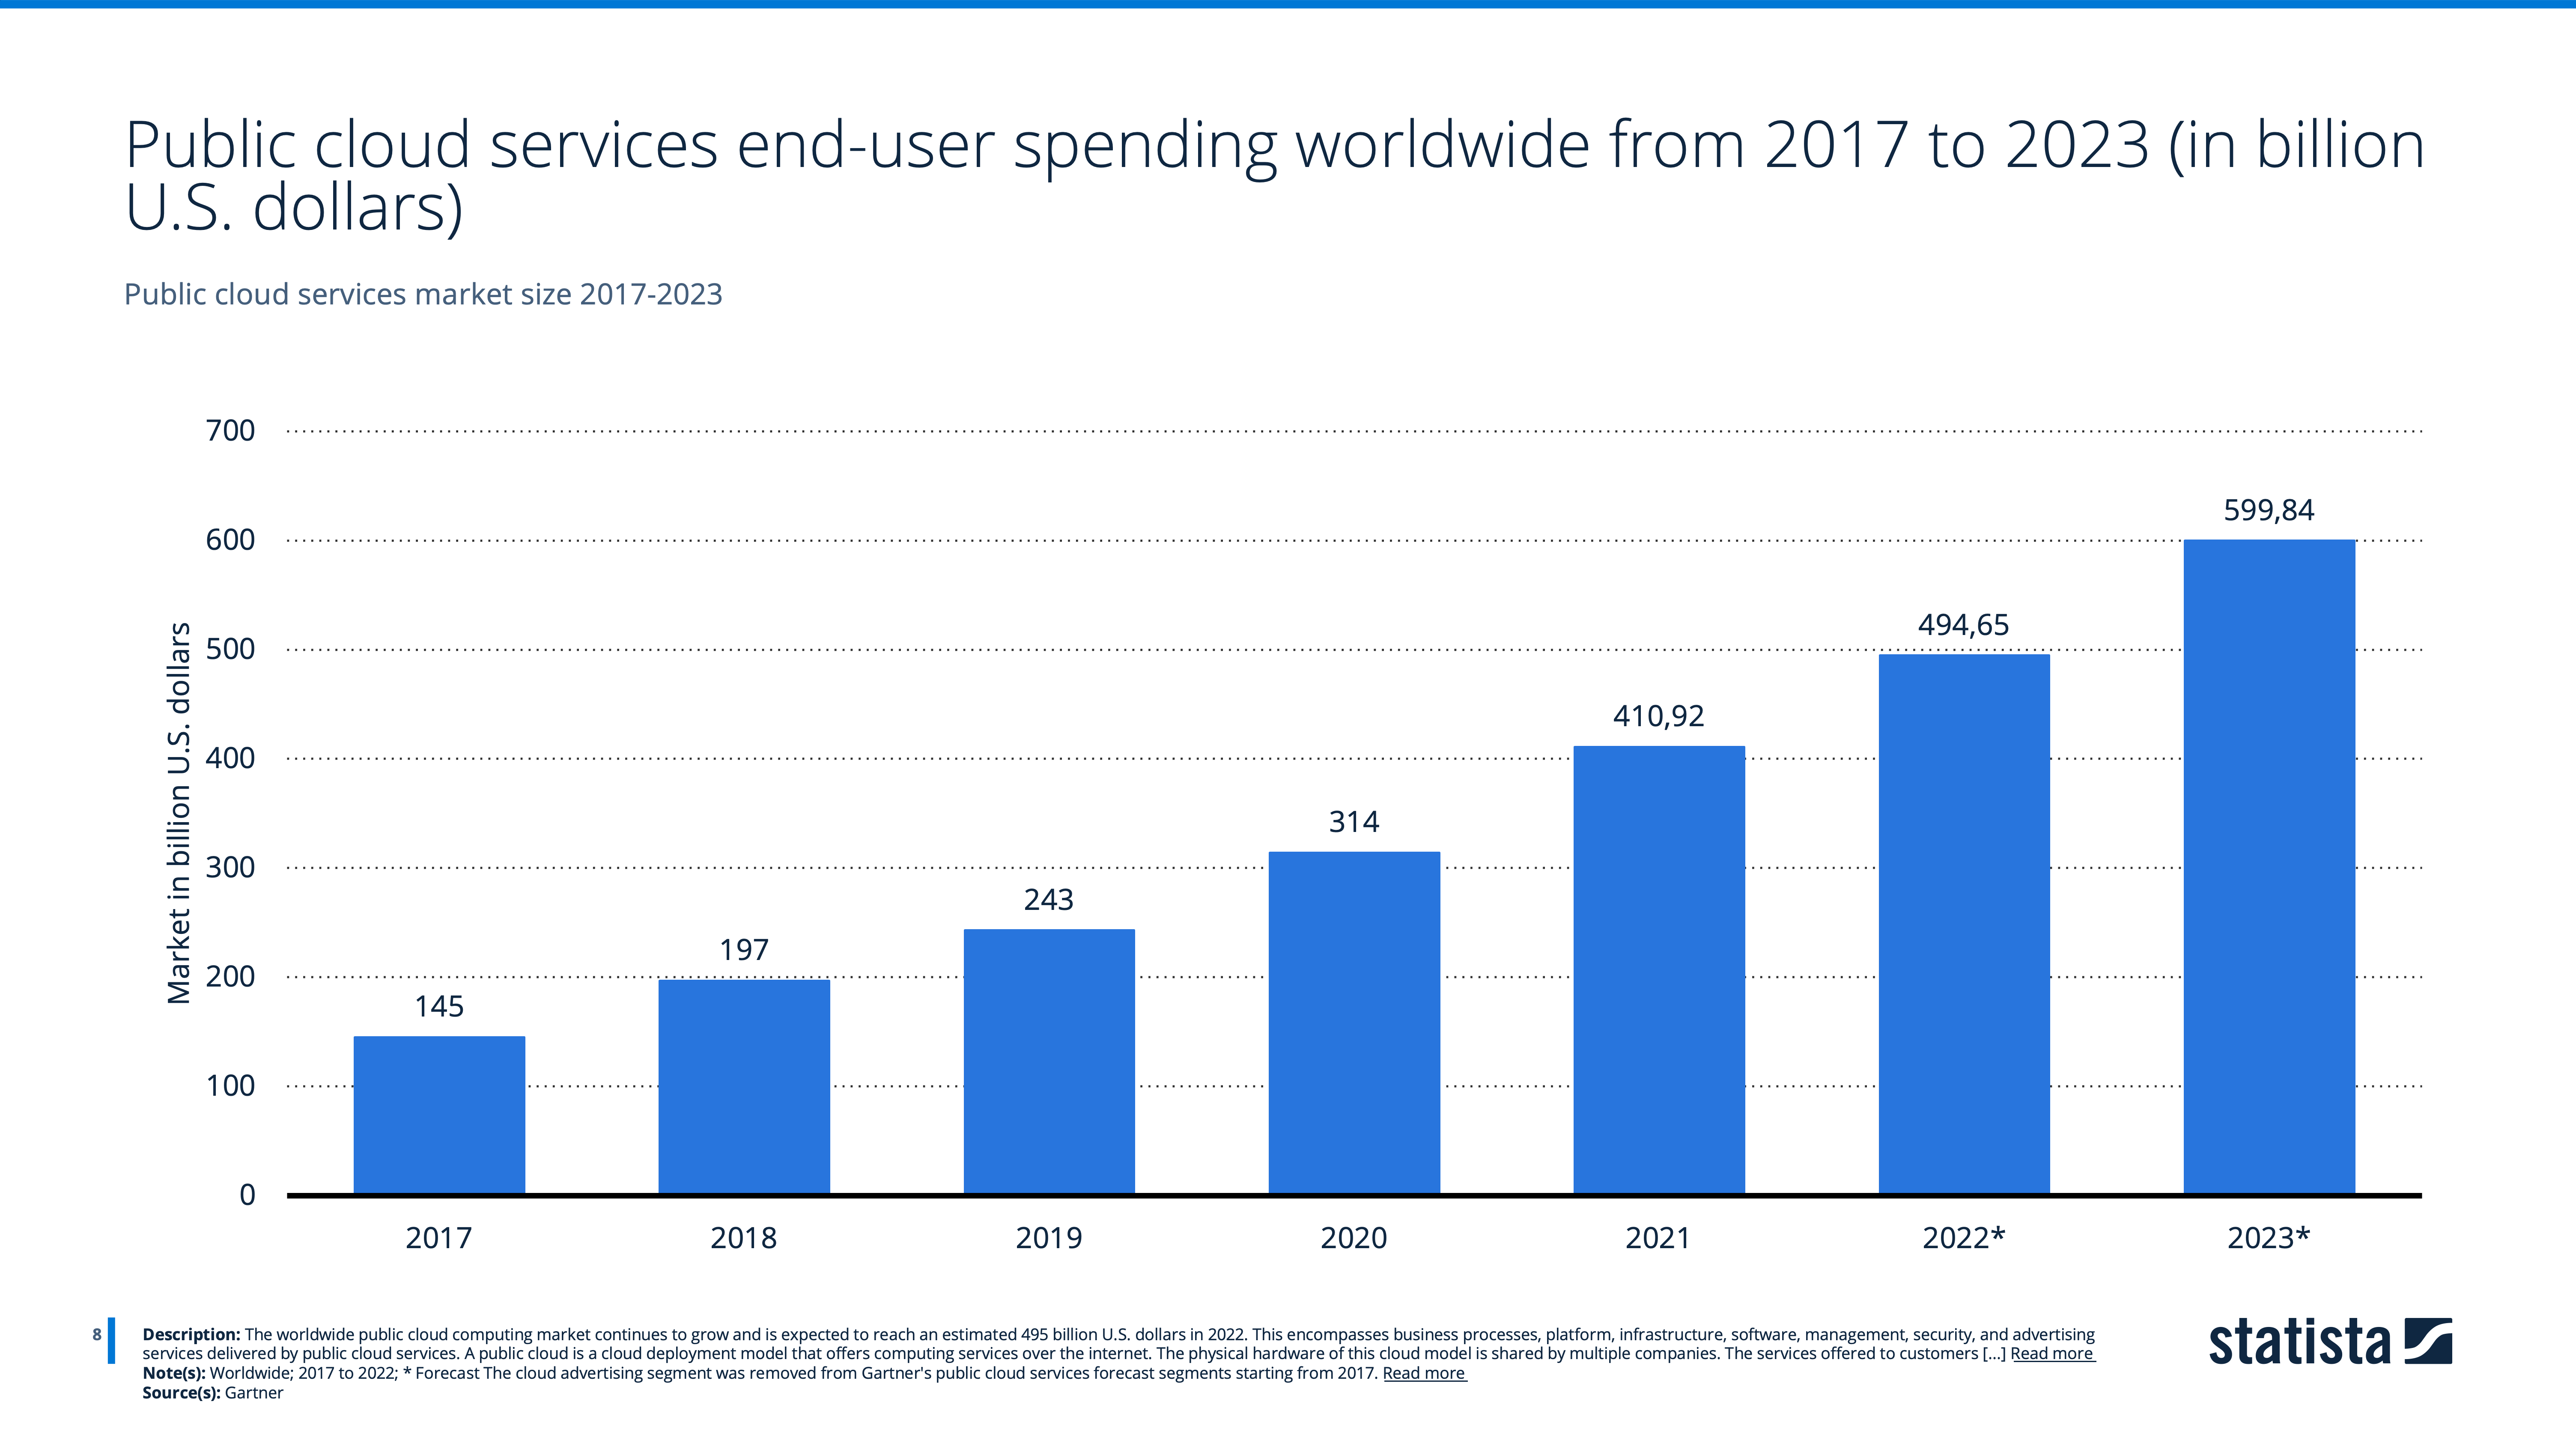
\includegraphics[width=\textwidth]{public_cloud_spending.png}
    \caption{Die Verkaufsleistungen der Public Cloud in den letzten Jahren \cite[S. 8]{Statista2022}}
    \label{fig:public_cloud_spending}
\end{figure}

Aus einem Dossier von Statista 2022 geht in der in Abbildung \ref{fig:public_cloud_spending} gezeigten Statistik hervor, dass sich die Ausgaben für Public Cloud Services von 2017 bis 2023 etwas mehr als vervierfacht haben werden \cite[Vgl.][S. 8]{Statista2022}. Auch weitere Statistiken desselben Dossiers machen einen stetig steigenden Trend hinsichtlich des Cloud Computing deutlich \cite[Vgl. unter anderem][S. 11ff]{Statista2022}. 

\pagebreak